% template.tex, dated April 5 2013
% This is a template file for Annual Reviews 1 column Journals
%
% Compilation using ar-1col.cls' - version 1.0, Aptara Inc.
% (c) 2013 AR
%
% Steps to compile: latex latex latex
%
% For tracking purposes => this is v1.0 - Apr. 2013
\documentclass{ar-1col}
\addtolength{\voffset}{-0.5in}
\addtolength{\hoffset}{-0.5in}

\usepackage{subcaption}
\usepackage{amsmath,amssymb}
\usepackage{amsfonts}
\usepackage{ulem}
\usepackage{natbib}
\usepackage{float}
\usepackage[hidelinks]{hyperref}

\setcounter{secnumdepth}{4}

% Metadata Information
\jname{Xxxx. Xxx. Xxx. Xxx.}
\jvol{AA}
\jyear{YYYY}
\doi{10.1146/((please add article doi))}

% macros
\newcommand{\g}[1]{{\color{blue}{#1}}}
\newcommand{\plr}[1]{{\color{green}{#1}}}
\newcommand{\triage}[1]{{\sout{\color{magenta}{#1}}}}
\newcommand{\todo}[1]{{\textbf{\color{red}{#1}}}}
\renewcommand{\emph}[1]{{\textit{#1}}}
\newcommand{\E}{\mathbb{E}}
\renewcommand{\P}{\mathbb{P}}


% Document starts
\begin{document}

% Page header
\markboth{Bradburd and Ralph}{Spatial Population Genetics}

% Title
\title{Spatial Population Genetics: It's About Time}


%Authors, affiliations address.
\author{Gideon S. Bradburd,$^1$ Peter L. Ralph$^2$
\affil{$^1$Ecology, Evolutionary Biology, and Behavior Group, Department of Integrative Biology, Michigan State University, East Lansing, MI, USA, 48824;
email: bradburd@msu.edu}
\affil{$^2$Institute of Ecology and Evolution, Departments of Mathematics and Biology, University of Oregon, Eugene, OR 97403}
}

%Abstract
\begin{abstract}
    Many questions that we have about the history and dynamics of organisms
    have a geographical component:
    How many are there, and where?
    How much do they interbreed across the landscape?
    How were they moving a thousand years ago,
    and where did the ancestors of an individual today live?
    Answers to these questions can have profound consequences
    for our understanding of history, ecology, and the evolutionary process.
    In this review, we discuss ways that geographic aspects of the 
    distribution, movement, and reproduction of organisms
    are reflected in their pedigree across space and time.
    Our aim is to provide intuition for how these processes,
    and variation in their action over time,  
    leave an imprint in genetic data,
    as the structure of the pedigree is what determines 
    patterns of relatedness in modern genetic variation.
    We also highlight some current methods and gaps 
    in the statistical toolbox of spatial population genetics.
\end{abstract}

%Keywords, etc.
\begin{keywords}
population genetics, geographic variation, isolation by distance, pedigree
%keywords, separated by comma, no full stop, lowercase
\end{keywords}
\maketitle

%Table of Contents
\tableofcontents

% Heading 1
\section{Introduction}

The field of population genetics is shaped by a continuing conversation
between theory, methods, and data.
We design experiments and collect data
with the methods we will use to analyze them in mind, 
and those methods are based on theory
developed to explain observations from data.
With some notable exceptions,
especially the work of Sewall Wright \citep{Wright1940,Wright1943,wright1946isolation}
and Gustave Mal\'ecot \citep{malecot}
much of the early body of theory was focused on
developing expectations for discrete populations.
This focus was informed by early empirical datasets,
most of which
(again, with exceptions \citet[e.g.,][]{Dobzhansky_Wright1943, dobzhansky1947}),
were well-described as discrete populations --
like samples of flies in a vial \citep{lewontin1974}.
For example, 
the first revolutionary empirical measurements
of molecular genetic variation \citep{HubbyLewontin66,LewontinHubby66}
% -- the inaugural ``find 'em and grind 'em" studies of Lewontin and Hubby \citep{HubbyLewontin66,LewontinHubby66} --
focused on data from 43 fly strains sampled from 5 locations,
which were treated as experimental replicates
(rather than studied in their geographic context).
In turn, 
the statistics used to analyze these datasets --
e.g., empirical measurements of $F_{ST}$ \citep{Wright1951}
or tests of Hardy-Weinberg equilibrium \citep{hardy1908,weinberg1908} --
were defined based on expectations in discrete, well-mixed populations.
In part, this was because much more detailed mathematical predictions 
were possible from such simplified models.
This focus of theory and methods on discrete populations in turn influenced
future sampling designs.

To what degree does reality match this picture
of clearly delimited yet randomly mating populations?
% In reality, well-delineated demes or clearly defined discrete populations are rare.
Often, the answer is: not well.
Organisms live, move, reproduce, and die,
connected by a vast pedigree that is anchored in time and space.
But, it is difficult to collect data and develop theory and methods
that capture this complexity.
Sampling and genotyping efforts are limited by time, money, and access.
Developing theory to describe evolutionary dynamics
without the simplifying assumption of random mating
is more difficult.
For example, without discrete populations,
many of the fundamental quantities in population genetics -- 
migration rate ($m_{ij}$), 
effective population size ($N_e$),
admixture proportion
--
are poorly defined.
Despite these difficulties,
there is now a growing body of theory, methods, and data
that approach this biological, population-less reality.
Today's large genomic datasets
are facilitating the estimation of the timing and extent of shared ancestry 
at a much finer geographic and temporal resolution than was previously possible
\citep{Li_Durbin2011,Palamara_2012,Harris_Nielsen_2013,ralph2013geography}.
And, advances in theory in continuous space 
\citep{felsenstein1975pain,BartonWilson1995,barton-depaulis-etheridge, barton2010modelling, barton2010newmodel, Barton2013},
datasets of unprecedented geographical scale
\citep[e.g.,][]{POBI, Aguillon2017deconstructing, Shaffer195743},
new computational tools for simulating spatial models \citep{haller2018forward,haller2018treesequence},
and new statistical paradigms for modeling those data 
\citep{petkova2016visualizing, ringbauer2017inferring, ringbauer2018estimating, conStruct, alasadi2018estimating}
are together bringing an understanding of the geographic distribution of genetic variation into reach.

The goal of this review
is to frame some of the fundamental questions in spatial population genetics,
and to highlight ways that new datasets and statistical methods 
can provide novel insights into these questions.
In the process, 
we hope to provide an introduction for empirical researchers
to the field.
We focus on a small number of foundational questions 
about the biology and history of organisms we study:
where they are; how they move; where their ancestors were;
how those quantities have changed over time, 
and whether there are groups of them.
We discuss each question
as a spatial population genetic problem, 
explained using the 
population's genealogy embedded in geographic space,
i.e., the \emph{spatial pedigree}.
% which we introduce as a powerful heuristic and an organizing principle for the field.
It is our hope that by framing our discussion around the spatial pedigree, 
we can build intuition for --
and spur new developments in --
the study of spatial population genetics .


%%%%%%%%%%%%%%%%%%%%%%%%%%%%%%
\section{The spatial pedigree}

The spatial pedigree 
encodes parent-child relationships of all individuals in a population,
both today and back through time,
along with their geographic positions (Figure \ref{spatial_pedigree}).
If we had complete knowledge of this vast pedigree,
we would know many evolutionary quantities
that we otherwise would have to estimate from data,
such as the true relatedness between any pair of individuals,
or each individual's realized fitness.
If we wanted to characterize dispersal behavior of a species,
we could simply count up the distances between offspring and their parents.
Or, if we wanted to to know whether a particular allele
was selected for in a given environment,
we could compare the mean fitness of all individuals in that environment with that allele
to that of those without the allele.

The ``location'' of an individual can be a slippery concept,
depending on the biology of the species in question
(as can the concept of ``individual'').
Where in space does a barnacle hitchhiking on a whale live, 
or a huge, clonal stand of aspen?
%In cases of doubt,
%remember it is actually the passage of genetic information that concerns us:
%the location at a particular time of the ancestor of a particular bit of DNA
%is much less ambiguous.
To reduce ambiguity,
we will think of the location of an individual as the place it was
born, hatched, or germinated.

\begin{figure}
    \centering
         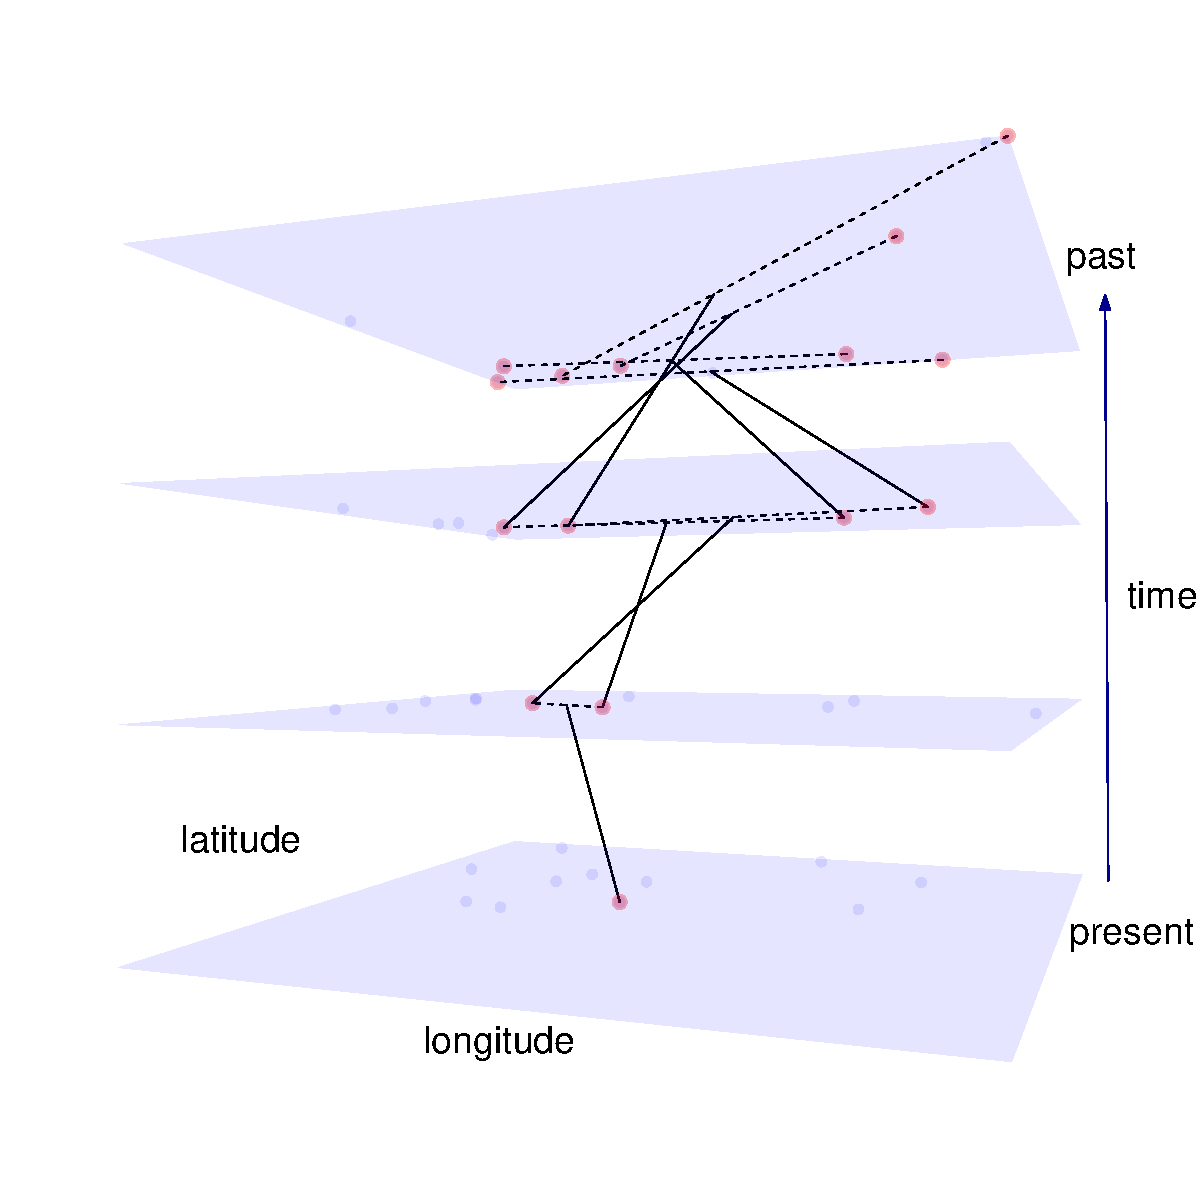
\includegraphics[width=\linewidth]{figs/spatial_pedigree.pdf}
        \caption{
		An example pedigree (left) of a focal individual sampled in the modern day, 
	   	placed in its geographic context to make the spatial pedigree (right).
		Dashed lines denote matings, and solid lines denote parentage.
		In the spatial pedigree, 
		each plane represents a a sampled region in a discrete (non-overlapping) generation,
		and each dot represents an individual.
		The pedigree of the focal individual is highlighted in red 
		back through time and across space.
        }
        \label{spatial_pedigree}
\end{figure}


In practice, we can never be certain of the exact spatial pedigree.
Even if we could census every living individual in a species
and establish the pedigree relationships between them all,
we still would not know about relationships between
and locations of individuals in previous, unsampled generations.
And, in a highly dispersive species,
or a species with a highly dispersive gamete,
there may be only a weak relationship between observed location and birth location.

Despite these complexities,
the idea of the spatial pedigree is useful
as a conceptual framework for spatial population genetics.
Although it may be difficult or impossible
to directly infer the spatial pedigree,
we can still catch glimpses of it through the window of today's genomes.

%%%%%%%%%%%
\subsection{Simulating spatial pedigrees}

It has only recently become possible to simulate whole genomes
of reasonably large populations
evolving across continuous geographic landscapes.
Throughout this paper, 
we illustrate concepts we discuss with simulations 
produced using SLiM v3.1 \citep{haller2018forward},
which enables rapid simulation of complex geographic demographies.
We recorded the genealogical history along entire chromosomes
of entire simulated populations
as a \emph{tree sequence} \citep{kelleher2018efficient},
and then used tools from \texttt{tskit} to extract relatedness information \todo{ref for tskit? is it just msprime?},
plotting the results in \texttt{python} with \texttt{matplotlib} \citep{hunter2007matplotlib}.
Our code is available at \url{https://github.com/gbradburd/spgr}.
This new ability to not only simulate large spatial populations,
but also to record entire chromosome-scale genealogies,
and thus ground-truth methods using actual spatial pedigrees,
has great promise for the field moving forward.


%%%%%%%%%%%
\subsection{``Effective'' parameters and the spatial pedigree}

\begin{quote}
    \textit{
    On one hand, every single one of my ancestors going back billions of years
    has managed to figure it out.
    On the other hand, that's the mother of all sampling biases.}
    \hfill \textit{-- Randall Munroe, xkcd:674}
\end{quote}

%There will be a recurring tension in this review
%between what we would like to know about (the spatial pedigree)
%and what we have information about 
%(the portion of it through which modern individuals have inherited genomes).
Inferences about the past
based on those artifacts that have survived to the present
are fraught with difficulties and caveats in any field, 
and population genetics is no exception.
The ancestors of modern-day genomes are \textit{not} an unbiased sample
from the past population -- 
they are biased towards individuals with more descendants today.
We cannot, of course, learn anything from modern-day genomes
about populations that died out entirely.
There are more subtle biases:
if we trace back the path along which a random individual today 
has inherited a random bit of genome,
the chance that a particular individual living $T$ units of time ago is an ancestor
is proportional to the amount of genetic material that individual has contributed to the modern population.
If we are looking one generation back, 
this is proportional to their number of offspring, i.e., their fitness.
If we are looking a long time in the past
(in practice, more than 10 or 20 generations \citep{BartonEtheridge2011fitness}),
this is their \textit{long-term fitness}.
Different methods query different time periods of the pedigree,
and are thus subject to these effects to different degrees.

A familiar example of this distinction is the difference between ``census'' and ``effective'' population size
\citep{Charlesworth2009}.
More subtle is the difference between dispersal distance ($\sigma$) and
``effective dispersal distance'' ($\sigma_e$) \citep{Cayuela2018demographic},
%% Does Cayuela really discuss sigma_e?
the quantity most naturally estimated from genetic data.
Both are mean distances between parent and offspring:
$\sigma$ is the average observed from, say, the modern population,
but $\sigma_e$ is
the mean distance between parent and offspring along a lineage back through the spatial pedigree.
The difference arises because
lineages along which genetic material is passed do not give an unbiased sample of all dispersal events;
they are weighted by their contribution to the population.
For instance, if there is strong local intra-specific competition,
individuals that dispersed farther from their parents (and their siblings)
may have been more likely to reproduce and therefore more likely to be ancestors of today's samples,
which would make $\sigma_e > \sigma$.
On the other hand, if there is substantial local adaptation,
many individuals may be dispersing to habitats dissimilar to that of their parents
and are unlikely to transmit genetic material to the next generation
because they are maladapted to the local environment,
and so $\sigma_e < \sigma$
\citep[for a review, see][]{wangbradburd2014}.


%%%%%%%%%%%%%%
\section{Things we want to know}

%%%%%%%%%%%%%%
\subsection{Where are they?}


Perhaps the first things we might use
to describe a geographically distributed population
are an estimate of the total population size,
and a map of population density across space.
Quantifying abundance and how it varies
can be crucial, e.g., for understanding
what habitat to prioritize for conservation \citep{zipkin2018synthesizing}, 
which regions have higher population carrying capacities than others \citep{roughgarden1974}, 
or whether a particular habitat is a demographic source or sink 
\citep{pulliam1988sources}.
The best measure of population density
would be a count of the number of individuals occurring in various geographic regions, 
and the best measure of total population size would be the sum of the counts across all regions.
How close can population genetics get us to estimating these quantities by indirect means?
Some fundamental limitations are clear:
for instance, if we only sample adults,
we cannot hope to estimate the proportion of juveniles that die before adulthood.
None of our sampled genetic material inherits from these unlucky individuals,
so they are invisible as we move back through the pedigree.
In addition, it is tricky to separate the inference of population density 
from that of dispersal, 
as the rate of dispersal to or from a region of interest 
governs whether it makes sense to consider the pedigree in that region on its own.
Partly because of this issue, 
it is also difficult to estimate total size from a sample of a 
non-panmictic population, 
and so it is more intuitive to discuss local density first, 
then scale up to the problem of total population size.
The spatial pedigree contains a record of both total and regional population sizes, 
and we can use data generated on it to learn about these quantities.


\begin{figure}	%[h]
    \centering
    \begin{subfigure}{0.95\textwidth}
        \centering
        \includegraphics[width=\linewidth]{figs/valley_density}
        \caption{map of simulation scenario}
        \label{valley_map}
    \end{subfigure}
    \begin{subfigure}{0.95\textwidth}
        \centering
        \includegraphics[width=\linewidth]{figs/valley_heterozygosity}
        \caption{individual heterozygosity}
        \label{valley_het}
    \end{subfigure}
        \caption{
            \textbf{(left)} Map of population density of the simulated population scenario
            we use for examples throughout.
            Populations have local density-dependent regulation
            within two valleys with high local carrying capacity (indicated by contours),
            separated and surrounded by areas with lower carrying capacity.
            The western valley has a carrying capacity about twice as large as that of the eastern valley.
            \textbf{(right)} Heterozygosity of a sample of 100 individuals across the range.
            Circle sizes are proportional to heterozygosity,
            and circle color indicates relative values
            (green: above the mean; white: mean; purple: below the mean).
            Low heterozygosities occur on the edges of the range,
            and average about 40\% lower in the lower-density eastern valley.
		}
        \label{pop_density}
\end{figure}



%%%%%%%%%%%%%%
\subsubsection{Population density}

Genetic information about population sizes or densities most clearly
comes from numbers and recency of shared ancestors, 
i.e., the rate at which coalescences are encountered moving back through the pedigree.
The relationship between density and coalescence is, in principle, straightforward:
with fewer possible ancestors,
individuals' common ancestors tend to be more recent.
To build an intuition for the effect of density on relatedness,
it is helpful to consider 
the problem of inferring the total size of the previous generation
in a randomly-mating population
from the number of siblings found in a random sample of size $n$.
There are $x (x-1) / 2$ sibling pairs in a family with $x$ offspring,
so the probability that, 
in a population of size $N$, 
a given pair of individuals are siblings
is $\E[X (X-1)] / (N-1)$, where $X$ is the number of offspring in a randomly chosen family.
This implies that in a sample of size $n$,
$n(n-1)/2$ divided by the number of observed sibling pairs 
provides an estimate of inbreeding effective population size, $N_e = N/\E[X(X-1)]$.
In other words, we should be able to use relatedness to estimate population size
up to the factor $\E[X(X-1)]$, which depends on demographic details. 
% Common ancestors -- i.e., coalescences --
% further back in time are simply more remote sibling pairs.
% so this calculation applies to estimates further in the past.
This same logic can be applied locally:
the (inbreeding) effective population density
near a location $x$, denoted $\rho_e(x)$,
can be defined as the inverse of the rate of appearance of sibling pairs
near $x$, per unit of geographic area and per generation.
This discussion is mostly illustrative, because
if a dataset does contain very many siblings,
nonrandom sampling is probably the cause,
and direct mark-recapture methods would often be more efficient.

However, we can extend this line of reasoning to see that 
the local density of close relatives
should reflect local population size.
The chance that two geographic neighbors actually \textit{are} siblings 
decreases with the number of ``possible nearby parents'':
\citet{wright1946isolation} quantified this with the
\emph{neighborhood size}, 
$N_\text{loc} = 4 \pi \rho_e \sigma_e^2$,
where $\sigma_e$ is the effective dispersal distance (discussed below)
and $\rho_e$ is the effective population density.
Each pair of siblings gives a small amount of information
about population density within distance $\sigma_e$ of the pair.
The more distant the coalescent event relating a pair of individuals, 
the vaguer the information they provide about population density,
because there is greater uncertainty 
both in the inference of their precise degree of relatedness from genetic data,
and in the location of their shared ancestors.
Because genetic estimates of population size 
derive from rates of coalescence,
they generally can only estimate population sizes 
in the locations and times where those coalescences occur.
% The lineages in the pedigree 
% of a geographic region that acts as a population ``sink'' 
% may tend to recently derive from a nearby ``source'' area,
% so that rates of coalescence depend more on the population size in the source area
% than on that in the entire range.

%%%%%%%%%%%%%%
\subsubsection{Total population size}

Estimates of the largest geographic scale -- total population size --
turn out to be sensitive to changes over the longest time scales.
Total effective population size is often estimated using measures of genetic diversity such as $\pi$ \citep{NeiLi1979,Tajima89},
the mean density of nucleotide differences between two randomly sampled chromosomes.
Because each such difference is the result of a mutation
sometime since the chromosomes' most recent common ancestor at that location on the genome,
$\pi$ is equal to twice the mean time to most recent common ancestor
within the sample, multiplied by the mutation rate.
In other words, if the per-nucleotide mutation rate is $\mu$,
and $2T$ is the mean length of a path through the pedigree
along which two samples have inherited a random bit of genome
from their most recent common ancestor,
then $\pi \approx 2 T \mu$.
The quantity $T$ itself is an interesting summary of the pedigree,
and depends on geography, sampling, and dispersal in complex ways;
what does it have to do with population size?
In a randomly mating, diploid population of constant effective size $N_e$,
the discussion above implies that $T = 2N_e$.
In practice, populations are rarely constant, and so this is viewed as an average
over the last few $N_e$ generations.


%%%%%%%%%%%%%%
\subsubsection{Example: Heterozygosity and population density}
\g{feels like this is too long, but also feels like it's good to, y'know, \emph{review} some stuff}
\plr{nice addition; maybe the wrong place? I've re-intro'ed this section; if you go with it, it needs a new title.}

Local population size is reflected in the pedigree through rates of shared ancestry:
all else being equal, smaller populations should have less genetic diversity.
To gain intuition, we will look at this idea in a simulated example.
Consider two adjacent valleys, 
one densely populated, the other sparsely populated, 
but both equal in geographic area 
and separated by a barrier to dispersal (Figure \ref{pop_density}\subref{valley_map}).
In general, we expect pairs of individuals in the low density valley 
to have shared ancestors in the more recent past than 
pairs of individuals in the densely populated valley.
This happens simply because 
each group of siblings makes up a larger proportion 
of the more sparsely populated valley.
Individuals in the sparsely populated valley 
have more shared ancestors in the more recent past, 
so the two chromosomes sampled in a each individual 
from that valley are more closely related,
i.e., have lower heterozygosity, as shown in Figure \ref{pop_density}\subref{valley_het}.

Does heterozygosity predict relative population density more generally?
Differences in heterozygosity can be shaped by other forces.
For example, we might also expect a similar difference in heterozygosity
if the two valleys had the \textit{same} population density per unit area,
but one valley was larger than the other,
because heterozygosity reflects population size.
Or, if dispersal distances tend to be shorter
in the more densely populated valley -- 
e.g., because resources are more plentiful, 
so that individuals do not have to disperse as far to find food -- 
there may be more inbreeding over short distances,
despite higher genetic diversity within the valley as a whole.

Migration into and out of a region presents another complication.
Roughly speaking,
geographic patterns of relatedness
are determined by a tension between population size and migration.
Genealogical relationships form on a time scale determined by population density,
because in a geographic region containing $N$ individuals
the chance that two individuals are siblings is of order $1/N$.
Shared ancestry is spatially autocorrelated
to the extent that this process of coalescence
occurs more quickly than migration.
If the migration rate into a geographic region is much greater than $1/N$ --
i.e., if more than a few individuals in each generation had parents living outside of the region --
then the pedigree in a region cannot be considered autonomously.
In other words,
regions cannot be analyzed independently
unless a region of interest sees less than one migrant per generation
(i.e., outside the parameter regime of the structured coalescent \citep{nagylaki1998}).

\plr{I think this should be moved up to the end of the local pop density section,
    because it reiterates several things there.}
There are two main alternative approaches to estimating local density: 
measuring the rate of genetic drift  and identifying close relatives \citep{Wang2016Prediction}.
To measure the rate of genetic drift, 
a researcher compares allele frequencies
in at least two samples collected in a region in different generations, 
either at different points in time,
or, in a species with overlapping generations, 
between contemporaneous individuals of different life stages
\citep{WilliamsonSlatkin1999}.
The rate of drift is governed by, 
and therefore provides an estimate of, 
local population size
\citep{ewens2004mpg,Charlesworth2009}.
Alternatively, a researcher can use a large sample in a single generation 
and leverage multilocus genotypes \citep{nomura2008estimation,WaplesWaples2011,Wang_2014},
shared rare alleles \citep{NovembreSlatkin2009}, 
or long shared haplotypes \citep[e.g.,][]{ralph2013geography}
to identify close relatives, like sibs, half-sibs, or recent cousins.
As discussed above, the proportion of identified close relatives out of the total (unbiased)
sample can inform an estimate of the local population density.
Because these latter approaches are pinned to the recent past, 
either by the generations sampled or by the degree of closeness of relatives,
they may offer a more accurate estimate of population density than heterozygosity does, 
especially when density has changed over time.
\g{more on this and about how heterozygosity reflects historical avgs?}


%%%%%%%%%%%%%%%%%%%%%%%%%%%%%%
\subsection{How do they move?}

Dispersal is fundamental to many questions in ecology and evolution,
such as
predicting the spread of pathogens \citep{BiekReal2010},
responses to climate change \citep{parmesan2006},
or population demography and dynamics \citep{schreiber2010interactive}.
We define dispersal to be the process that governs 
the displacement between geographic locations of parent and offspring.
%but combines many important aspects of the organism's ecology, including
%any movement of gametes or zygotes before maturation,
%and subsequent daily or seasonal movement of the mature individual,
%all of which often depend on the sex of both parent and offspring.
For some species,
it may be feasible to directly measure dispersal 
using, e.g., telemetry or banding \citep{Cayuela2018demographic},
but this is often prohibitively expensive or difficult.
Although we usually do not know the spatial locations of ancestors in the pedigree,
the spatial locations of modern individuals can give strong clues about this.


%%%%%%%%%%%%%%
\subsubsection{Dispersal (individual, diffusive movement; $\sigma$)}

We call the absolute value of the spatial displacement between parent and offspring locations
the \textit{dispersal distance}, and refer to it as $\sigma$.
The dispersal distance describes the quantity one could calculate by,
e.g., collecting a large number of germinating seeds
and averaging the distance from those seeds to their two parents.
It determines how quickly spatial populations mix.

Dispersal distance could be trivially estimated by taking
the average of these displacements across history
if we knew the spatial pedigree through time without error.
In practice, we often are only able to directly observe
the location of individuals in the present day.
However, 
spatial distances between individuals of different levels of relatedness
give us information about dispersal distance, even without parental locations.
This spatial clustering of close relatives
is shown in Figure \ref{fig:dispersal}\subref{cousin_map}.
For example,
the distance between siblings is the result of two dispersals,
so an average of this distance over many pairs of siblings 
gives an estimate of $2 \sigma$.
The mean squared displacement along
a path of total length $n$ through the pedigree is $\sigma^2 n$:
first cousins would give four times the dispersal distance, and so forth.
% assuming that $n$ is short enough that boundary effects can be ignored.
Unfortunately, basing an estimator of $\sigma$ on this observation
is is usually infeasible in practice,
unless a large fraction of the population has been genotyped
\citep[e.g.,][]{Aguillon2017deconstructing}.

Instead of identifying close relatives,
we might use the decay of mean genetic relatedness with distance
(shown in Figure \ref{fig:dispersal}\subref{ibd}).
The mean time since most recent common ancestor 
of two individuals at a random point on the genome
is usually larger for more distant individuals \citep{ibd_review},
a relationship that clearly has something to do with $\sigma$.
An approximate formula for this relationship
in homogeneous space (Malec\'ot's formula)
can be derived in various ways 
\citep{malecot, sawyer1976branching, rousset_1997, barton-depaulis-etheridge, robledoarnuncio, ringbauer2017inferring, alasadi2018estimating},
but is composed of two parts: 
(a) how long has it been since the two individuals last had ancestors that lived near to each other,
and (b) how long before that did they actually share an ancestor.
The second part is not well understood,
but \citet{malecot} assumed that the second stage acts as in a randomly mating population
with some local effective size, $N_\text{loc}$.


\begin{figure}	%[H]
    \centering
    \begin{subfigure}{0.85\textwidth}
        \centering
        \includegraphics[width=\linewidth]{figs/valley_cousins.pdf}
        \label{cousin_map}
    \end{subfigure}
    \begin{subfigure}{0.75\textwidth}
        \centering
        \includegraphics[width=\linewidth]{figs/valley_ibd.pdf}
        \label{ibd}
    \end{subfigure}
    \begin{subfigure}{0.85\textwidth}
        \centering
        \includegraphics[width=\linewidth]{figs/valley_line_flux.pdf}
        \label{valleyflux}
    \end{subfigure}
        \caption{
            \textbf{(top)} Map of close genealogical relatives of four focal individuals.
            Geographic locations of 
            genealogical relatives are shown as larger dots, with one color for each focal individual,
            with circle area proportional to the expected proportion of genome shared
            (i.e., $2^{-k}$, where $k$ is the number of steps in the shortest path through the pedigree to the focal individual).
            \textbf{(middle)}
            Genetic against geographic distance between each of four focal individuals
            (colors the same as in the top figure)
            and 100 other individuals, from the same map as above.
            Genetic distance (calculated as expected sequence divergence)
            increases with geographic distance within and between each valley at similar rates,
            but levels off within each valley at different values
            due to different population sizes.
            \textbf{(bottom)}
            Flux across two boundaries on the same continuous map as above.
            All individuals across about 8 generations are shown as small dots,
            and every parent-child relationship that crosses each of the dotted lines
            is illustrated by an arrow, colored either red (if it crosses west-to-east) or blue (east-to-west).
        }
        \label{fig:dispersal}
\end{figure}

%%%%%%%%%%%%%%
\subsubsection{Dispersal flux}

Dispersal ability is not, of course, constant across real landscapes, and
we would often like to measure the ``amount of gene flow'' across some barrier
or between two geographic regions.
For some boundary (i.e., a line on the map),
we can ask for the number of dispersal events that cross it in a given year -- 
that is, 
how many individuals are born each year whose parents
were born on the other side of the line?
This quantity, which we call the \textit{dispersal flux} across the boundary,
is useful for investigating connectivity between different areas
and the role of the landscape in shaping patterns of dispersal.
Dispersal flux is a geographical analogue of
the ``migration rate'' between discrete, isolated populations. 
Note that dispersal flux is not constrained to be equal in both directions across a boundary:
it may be easier to disperse down-current than up-current.
For instance, Figure~\ref{fig:dispersal}C
shows the number of dispersal events crossing two lines on our simulated valley landscape
over a few generations.
The line on the west goes through the denser valley, 
and so has a large flux in each direction.
The eastern line goes along the edge of the sparser valley,
and so has lower flux overall, and more east-to-west flux
due to the higher population density to the east of the line.

As before, if we had complete knowledge of the spatial pedigree,
we could calculate the flux across any line simply by counting the number of
parent-offspring pairs that span it.
However, it is rare to find any one individual
that is a direct genetic ancestor of another in a dataset
(apart from perhaps some parent-child relationships).
As a result, we almost never infer a direct chain of dispersal events,
only dispersal since coalescence events.
The likely locations of these coalescent events
depends on the maps of population density and fecundity,
thus entangling
the problems of inferring dispersal flux and population density.

For instance, across a barrier with low flux,
the average time to coalescence for pairs of individuals on opposite sides of the line
is longer than that between individuals on the same side \citep{bedassle,Duforet-Frebourg_Blum_2014,ringbauer2018estimating}.
Flux across a line is also related to mean dispersal distance, $\sigma$, discussed above.
The expected flux across a straight boundary in a homogeneous area,
per unit time and per unit of boundary length,
is equal to the birth rate per unit area multiplied by $2 \sigma / \pi$
\citep{buffon1777},
so estimates of flux can be converted to estimates of dispersal distance.


%%%%%%%%%%%%%%
\subsubsection{Estimating dispersal and flux}

\begin{itemize}
\item How do we estimate effective dispersal and flux using genetic data? 
\subitem Fst and IM models, estimating gene flow (Slatkin 1985)
        \plr{we should mention the connection to $F_{ST}$ below in ``relative genetic differentiation''}
\subitem \citet{rousset_1997} used this formula to show that
the slope of $F_{ST}$ against the logarithm of distance
is under these assumptions an estimator for $4 \pi \rho_e \sigma_e^2$,
but it is not known to what degree the assumptions affect the results.
\subitem This general idea was applied to much larger time scales by \citep{neigel1991estimation,neigel1993application},
who used the genealogical tree relating many samples at one nonrecombining locus
(e.g., the mitochondria) and the spatial locations of these samples
to infer $\sigma$ using phylogenetic comparative methods.
\subitem however... see whitlock \& Mccauley
\item alternatively, identification of relatives using shared tracts of ancestry
\subitem (ralph and coop, palamara and pe'er, harris and nielsen, Ringbauer \& friends 2017)
\item maps of Isolation by Resistance 
    \citep{McRae2006,McRae_Beier_2007,McRae2008,petkova2016visualizing} 
    describes the effective ``resistance" to gene flow 
    between points in space due to heterogeneity 
    in an organism's ability to cross the intervening landscape.
\end{itemize}

\plr{Proposal: put back the section on spatial maps of dispersal (shorter?) 
    and use it as a segue say that we've got a start at this, they are called resistance surfaces,
    cite circuitscape, eems, maps, and Erik's paper. Unless we're too long.}


%%%%%%%%%%%%%%
\subsection{Where were their ancestors?}

Above, we have discussed how population dynamics of movement and reproduction
are reflected in the spatial pedigree.
A complementary view is to
start with individuals sampled in the present day,
then, looking backwards in time,
to ask where in space they have inherited their genomes from, 
i.e., where their ancestors lived.
Because the signal in genetic data comes from 
shared ancestry and coalescence in the pedigree,
thinking from this reverse-time perspective 
is useful in interpreting genetic data.
However, summaries of how ancestry spreads across space 
through the pedigree can be important in their own right.
For example, many humans are interested
in the locations of their own ancestors back in time.
More generally,
we are often also interested in the partitioning of genetic diversity across space,
e.g.,
quantifying the strength of inbreeding locally,
or assessing the capacity of a population to become locally adapted.
Spatial distributions of ancestry compared across sections of the genome
could also be informative about 
other processes, such as
the origins and mechanisms of selective sweeps.


%%%%%%%%%%
\subsubsection{Geographic distribution of ancestry}

\todo{estimation section? or parallel structure with other sections?}

As one looks further back in time,
the geographic distribution of an individual's ancestors
is determined by the history of population size changes and movements.
At any point in the past,
each portion of each individual's genome can be associated 
with the ancestor from whom they inherited it.
Their genetic ancestry can therefore be apportioned across space according
to the locations of the ancestors from whom they inherited their genome.
%There are a number of natural questions that arise from a description of this process.
%How much of an average individual's ancestry is still within a given region, 
%at some point in the past?
%How long in the past was it since a typical individual in one location had an ancestor
%in another geographic region (say, the next valley over)?
%How far back in time do you have to go before 
%the average proportion of ancestry that an individual inherits
%from the local region they live in drops below (say) 90\%?

This spatial distribution of \textit{all} genetic ancestors is depicted 
at several points back in time
for four individuals in a simulation in Figure~\ref{ancestry_spread}.
As we look further back in time,
we can see the ``cloud of ancestry'' spread out across space.
The spread is diffusive --
the mean displacement of a given $n^\text{th}$-generation ancestor 
is of order $\sigma_e \sqrt{n}$,
as long as this is small relative to the width of the region.
Not shown on the map are the many genealogical ancestors
from which the focal individuals have not inherited genome --
even by the second figure,
each focal individual is genealogically descended from nearly everyone alive,
even those living in the other valley \citep{chang1999}.

\begin{figure}	%[H]
        \includegraphics[width=0.75\linewidth]{figs/valley_ancestry_01.pdf}
        \includegraphics[width=0.75\linewidth]{figs/valley_ancestry_60.pdf}
        \includegraphics[width=0.75\linewidth]{figs/valley_ancestry_300.pdf}
        \caption{
            Spatial locations of the ancestors of four individuals:
            at 
            \textbf{(top)} one, 
            \textbf{(middle)} fifteen, and
            \textbf{(bottom)} seventy-five generations in the past.
            All individuals from whom the four individuals have inherited genome are denoted by a circle,
            with one color for each individual,
            and with circle area proportional to the amount of genome inherited.
            The landscape is the same as in Figure~\ref{fig:dispersal}.
            Since the simulation uses overlapping generations,
            ancestors of different degrees are present at the same time.
        }
        \label{ancestry_spread}
\end{figure}

Although Figure~\ref{ancestry_spread} does not highlight 
ancestors \textit{shared} by any pair of the focal individuals,
it is clear that these occur in the overlap between their two clouds of ancestry.
For instance, any ancestors shared over the time interval shown
between the pink and purple individuals
must be in the western valley,
and it is these shared ancestors that tell us about relative population densities in the two valleys.
In fact, we know from Figure~\ref{pop_density}B that these recent shared pink--purple ancestors
must represent a larger fraction of the genome
than do the orange--green shared ancestors.


%%%%%%%%%%%%%%
\subsubsection{Relative genetic differentiation}

In the ``two valley'' simulation of Figure \ref{ancestry_spread},
ancestors are shared within valleys over the time period shown,
but not between valleys.
The difference in the geographic distribution of shared ancestors 
results in higher relatedness between the pairs of individuals 
from the same valley, 
and it underlies all measurements of relative genetic differentiation.
The most common measure of
how much more closely related neighbors are to each other relative to the population as a whole
is $F_{ST}$ \citep{Wright1951},
which can be thought of as estimating
one minus the ratio of mean coalescence time within subpopulations
to that within the entire population \citep{slatkin_1991inbreeding}.
%-- a descriptor of average tree shape in the pedigree. 
The normalization by mean overall coalescence time 
makes this relative measure comparable across populations of different sizes.

In stationary populations,
relative genetic differentiation is determined by the tension between 
geographic mixing (due to dispersal flux between areas)
and local coalescence (determined by population density).
In the more remote past, each individual's ancestors are distributed across
all of geography,
so that the long-ago portion of the pedigree looks like that of a randomly mating population.
Tracing the pedigree backward in time, 
remote ancestors have ``forgotten" the geographic position of their 
modern-day descendants.
The transition between these two phases -- recent spatial autocorrelation 
(``scattering") and distant random mating (``collecting")
\citep{Wakeley1999,wilkins2004separationoftimescales}
happens on the time scale over which a lineage crosses the species range \citep{Wakeley1999}.
Since lineage motion is diffusive, in a continuous range of width $L \sigma_e$,
coalescences between lineages of distant individuals happen on a time scale of $L^2$ generations.
Relative genetic differentiation
is determined by the likelihood that coalescence between two nearby individuals
occurs during the scattering phase
-- i.e., by the length of time that two spatial clouds of ancestry of Figure \ref{ancestry_spread}
are correlated with each other,
relative to the local effective population size.

$F_{ST}$ may not be best measure of this quantity -- 
others are possible that depend less on the deep history of the population.
For instance,
one could ask for the proportion of the genomes of two neighbors 
inherited in common from ancestors int he last $T$ generations
relative to the same quantity for distant individuals,
where $T$ is chosen to reflect the time scale of interest.
The appropriate measure will depend on the application at hand.

%%%%%%%%%%%
\subsection{Clustering, grouping, and ``admixture''}

\plr{I think there's some redundancy below.}

Many tools for modern analysis of genetic data
partition existing genetic variation into clusters labeled as (discrete) populations
\citep[e.g.,][]{STRUCTURE, ADMIXTURE}
% Perched on the shoulder of discrete population structure is the concept of admixture,
% the idea that populations can be composed of ancestry from multiple discrete groups.
The ubiquity of gene flow means that
any conceptual model of discrete populations 
must also include \emph{admixture} between them.
Models of discrete population structure and admixture 
provide visualizations that can be helpful for
describing and making sense of patterns of relatedness and genetic variation.
Coupled with a quantification of relative genetic differentiation,
they can be used in conservation to delineate discrete management units.
However, in practice these discrete groups may easily be determined
by clustering of sampling effort,
calling into question their real-world interpretation.
Explicitly utilizing geographic proximity can help alleviate these concerns \citep{conStruct},
but it would still be desirable to delineate groups in a way explicitly linked
to the actual history of relatedness, i.e., the spatial pedigree.

The real-world situation when admixture between discrete populations 
is perhaps most clearly defined is when populations that have been completely separated
for a long period of time come back into contact.
In this case, the discrete populations are defined by partitioning \emph{ancestral} individuals,
and admixture of subsequent generations is determined by inheritance from them.
For instance, suppose that 
the two valleys of our running example
were isolated during a long period of ``glaciation'',
followed by glacial retreat and expansion into secondary contact.
The valleys clearly act as discrete populations during glaciation, 
during which there are are few if any pedigree connections between the valleys.
Pedigrees only start to overlap more recently between individuals in each valley.
To obtain an admixture proportion,
we can fix some ``reference'' time in the past,
and label each subsequent individual's genomes
according to which of the two valleys it inherited from at the reference time.
% The precise reference time does not matter as long as there was no gene flow during isolation.
This is shown in Figure \ref{postglacial_expansion}:
eight generations after contact (top),
this quantity clearly reflects the history of isolation;  
individuals in or near each valley have inherited most of their genomes 
from ancestors in the closest valley.
However, if we return 75 generations later, 
we see a more complicated story (bottom).
The continued spatial mixing has resulted in a significant 
portion of ancestry in the west valley inherited from 
glacial-era ancestors in the east valley, 
and vice versa.
Further complicating the issue, 
the west-to-east flux across the ridge between the valleys 
is higher than that in the opposite direction 
because the western valley has a higher population density. 
As a result, a much higher proportion of the genomes
in the eastern valley are now inherited 
from individuals that, 
during glaciation, were found in the western valley.

\begin{figure}	%[H]
    \centering
        \includegraphics[width=0.85\linewidth]{figs/valley_admixture_new}
        \includegraphics[width=0.85\linewidth]{figs/valley_admixture_old}
        \caption{
            Admixture proportions after a recent secondary contact.
            Each pie shows the proportion of a diploid individual's genomes
            that inherit from the western (red) and eastern (blue) valleys, respecitvely.
            \textbf{(top)} Eight generations, and
            \textbf{(bottom)} seventy-five generations 
            after a barrier along the top of the ridge is removed.
        }
        \label{postglacial_expansion}
\end{figure}

This simulation highlights both the relevance of 
a model of discrete population structure and admixture
to spatially continuous data, 
and also its limitations.
Using the period of glacial isolation as our reference point, 
it is straightforward to designate individuals in each valley 
as members of different populations 
(although note that, in the early stages of isolation, 
individuals in each valley may have had recent pedigree overlap, 
depending on the flux across the previously un-glaciated ridge).
Likewise, 
in the interval shortly after secondary contact, 
it is useful to visualize patterns of genetic variation 
by identifying the proportion of ancestry 
each individual derives from glacial-era ancestors in each valley.
However, 
outside the time during and immediately following glaciation, 
describing genotyped individuals on this landscape 
using a model of discrete populations with admixture 
becomes less helpful.
Without a concrete interpretation based in the population pedigree,
partitioning genetic variation into discrete groups, 
and labeling of samples as admixed between those groups
can encourage the incorrect interpretation that discrete populations are platonic ideals,
real and unchanging.
% As has been noted elsewhere 
% \citep{reich_india_2009,patterson_ancient_2012,hellenthal2014genetic,lawson2018tutorial},
% the power to infer a recent admixture event between historically separated populations
% is a function of the recency of admixture and
% the inclusion of populations descended 
% from the sources of admixture in the modern day sample.
% Indeed, the concept of admixture becomes slipperier when considered over deeper timescales,
% as populations inferred as sources of admixture are themselves almost certainly ``admixed,"
% and have either been isolated for long enough that the admixture is no longer detectable,
% or, more likely, the descendants of those sources of admixture are lost in the modern sample.

\g{estimating admixture?! could talk about the utility of chromosome painting etc.}

%%%%%%%%%%
\subsection{How have things changed over time?}

As we have discussed above,
different methods are sensitive to signal
from different time slices of the pedigree.
Of course, the geographic distributions and dispersal patterns of most species,
not to mention the landscape itself,
have changed over the time scale spanned by the pedigree of modern individuals.
For example, 
high-latitude tree populations may only have been established
following the retreat of the glaciers
a few tens of generations ago \citep{WhitlockMcCauley1999},
and invasive species may have entered their current
environment even more recently than that.
In addition to organisms moving themselves across landscapes,
landscapes are often changing out from under organisms' feet.

Anthropogenic land use
and global climate change
are radically altering both where organisms can live
and where they disperse \citep{parmesan1999}.
The result is that many empirical systems
are not in equilibrium,
so that the dynamics we estimate from
measurements of extant individuals may
not be representative of those in the past.
Exacerbating this problem,
it can take a long time to reach equilibrium
in areas of high population density
or across regions of low flux
\citep{CrowAoki1984group, whitlock1992temporal, slatkin1993isolation, WhitlockMcCauley1999}.
Theory and methods that can address change across both time and space
are still lacking,
and present an exciting set of challenges for the field.

%%%%%%%%%%
\subsubsection{Genealogical strata}

The field of population genetics
has many heuristics for which aspects of genetic data
contains information about older or more recent times in a population's history.
Rare alleles tend to be recent,
and long shared haplotypes even more so;
pairwise statistics like $\pi$ mostly inform us about events long ago,
on a scale of $N_e$ generations.
Different statistics thus provide us with windows into different strata of the pedigree.
Using rates of sibling- and cousin-ship,
the last few generations of history would be the easiest to understand,
but carries the perhaps unreasonable requirement of a sample 
that is a sizeable fraction of the entire population.
Methods for inferring the distant history of populations using a few samples
are the most well-developed \citep[e.g.,]{dadi,psmc,momi},
but these can incorporate very little in terms of geographic realism,
and indeed much of the signal of geography 
may have washed out on this coalescent time scale \citep{wilkins2004separationoftimescales}.
The length spectrum of long, shared haplotypes
(also known as IBD segments)
can be used to peer into the strata of the pedigree between these two time scales:
since the lengths of segments of genome inherited in common by two individuals
from $t$ generations ago scales roughly with $1/t$, 
these can carry substantial information about ancestors from only tens of generations ago.
This fact has been used by \citet{alasadi2018estimating}
to create estimated maps of population density and migration rate
for different, recent time slices.
However, the different strata cannot be read independently
-- the correspondence between shared haplotype length and age of common ancestor
depends strongly on population size history \citep{ralph2013geography}.


%%%%%%%%%%
\subsubsection{Now is the winter of our discontinuity}

\plr{shorten this up, I think, and call it something besides discontinuity? I have not heard this, and connotes other things to me.}

The specter of \textit{spatial discontinuity} --
the phenomenon in which none of the individuals 
living in a particular region at a particular point in time 
are descended from any of the individuals living in that region 
at some point in the past
-- haunts the inference of historical processes
from data genotyped from extant samples in an area.
Spatial discontinuity, 
also known as population replacement, 
can arise when regions become unoccupied
(e.g., due to ecological disturbance) 
and are recolonized by immigrants from elsewhere, 
or when agonistic interactions between immigrants and local individuals 
lead to local displacement. 
Assuming that nearby individuals are more related than distant individuals, 
the genetic signature of spatial discontinuity will be most pronounced 
when the immigrant genotypes are from far away.

Spatial discontinuity presents such a problem because 
inference of many of the quantities discussed above --  
e.g., local density, dispersal, and flux --
is predicated on the assumption that 
the observed geographic distribution of genetic variation 
was generated in the sampled geographic context.
For example, 
we assume that the flux across the ridge 
depicted in Figure \ref{fig:dispersal}\subref{valleyflux}
and inferred from observed divergence 
between samples in the two adjacent valleys 
is indicative of true dispersal across the ridge.
If, alternatively, one of the valleys 
has been recently colonized by individuals from elsewhere, 
the inferred effect of the ridge on dispersal may not reflect the truth.
Spatial discontinuity in a region is especially pernicious because, 
without genotyped ancient or historical individuals, 
it may be effectively invisible.

There is abundant evidence of spatial discontinuity 
from empirical datasets that include ancient or historical samples 
\citep{bi2013unlocking, skoglund2014investigating, PickrellReich2014, lazaridis_ancient_2014, haak2015massive, allentoft2015population, joseph2018inference}.
And, in many systems for which we have not yet genotyped historical samples, 
we have strong reason to suspect discontinuity 
because the local populations have been recently established 
following, e.g., glacial retreat or human-mediated invasions.
As we develop more datasets that include genotype data from historical individuals, 
we will better be able to evaluate the prevalence of spatial discontinuity 
and its effects on our inferences across natural systems. 


%%%%%%%%%%%
\section{Exciting directions for the field}

In this review we have focused on \emph{demographic inference} --
seeking to learn about past or present demographic processes
from population genetic data.
As demography -- birth, reproduction, death -- 
is the the mechanism by which natural selection occurs,
this is fundamental not only to history and ecology but also evolutionary biology.
Describing the geographic distribution of genetic variation -- 
its patterns, 
the processes that have generated and maintained it, 
and its consequences -- 
is a fundamental goal of evolutionary biology.
Below, we describe a few areas 
in which we hope or expect further progress in the field to be made.


%%%%%%%%%%%
\subsubsection{Selection}

Some of the most important aspects of geographic population genetics
we have not reviewed are related to natural selection.
Perhaps the most significant avenue for future work is to 
develop methods that jointly estimate selection and demography for spatially continuous populations. 
The questions introduced above are all presented in the context 
of a neutrally evolving population,
but clearly local adaptation and natural selection will impact 
the structure, and the spatial structure, of the pedigree.
There is a great deal known about the expected geographical action of selection,
e.g., how beneficial alleles spread across space \citep{fisher1932,hallatschek,ralph2010},
how locally adaptive alleles can be maintained in the face of gene flow \citep{slatkin_local,barton,ralph_patchy},
or how hybrid zones are structured \citep{barton_hybrid,sedghifar}.
In all these situations,
demographic processes have \emph{different effects} on different regions of the genome.
Incorporating selection into spatially continuous models 
will facilitate a greater union of population genetic processes 
and ecological models of population dynamics, 
and help shed light on important evolutionary questions.
% like where adaptive sweeps originate. 


%%%%%%%%%%%
\subsubsection{Simulation and inference} 

Spatial population genetics suffers from a singular lack of concrete mathematical results
that can be used for inference.
What can take its place?
A recent advance in the field, 
which may help improve inference models with and without selection, 
has been the advent of powerful and flexible simulation methods, 
such as SLiM \citep{haller2018forward,haller2018treesequence,kelleher2018efficient}.
These methods allow
researchers to simulate genome-scale datasets under models of arbitrary complexity.
This capability offers an excellent pedagogical tool 
and opportunity to build intuition for patterns of genetic variation 
in complex scenarios for which theory may be lacking.
% Indeed, we generated all figures for this paper using SLiM, 
% and we have included the simulations 
% and the code used to generate all figures 
% as an online supplement to our paper 
% (available for download at XXXX).
In addition, these simulation methods can be used in statistical inference.
For example, simulated datasets can be used in the training 
of machine learning methods \citep[e.g.,][]{SchriderKern2018}, 
or to compare between different generative models using 
approximate Bayesian computation \citep{MarjoramTavare2006modern}.
Simulation-based inference presents an exciting way forward 
for problems that may be analytically intractable.


%%%%%%%%%%
\subsubsection{Identifiability and ill-posedness}
\todo{keep?}

Another important gap in current methods for spatial population genetics inference 
is a quantitative understanding of the limits of our ability to learn about 
quantities of interest.
Demographic inference with population genetics data
is an example of an \emph{inverse problem} --
the mapping from parameters to data is relatively well-understood,
but the inverse map is not.
Many inverse problems are \emph{ill-posed},
meaning that many distinct models give rise to statistically indistinguishable datasets,
i.e., some degree of statistical nonidentifiability.
For example, 
as with effective population size \citep{Myers2008},
we may never be able to infer rapid changes in 
or reversals to effective population density
\citep[although see also][]{BhaskarSong2014descartes}.
Likewise, 
the timing of heterogeneity in flux across a particular part of the landscape 
may be difficult to disentangle from the magnitude of its change, 
as is the case with migration/isolation models 
of dynamics in discrete demes \citep{sousa2011nonidentifiability}.
More generally,
it may be difficult to learn about local biases in flux, 
or large-scale anisotropy in the direction of dispersal,
without genetic data from historical individuals 
that could be used to anchor the spatial pedigree 
in time and space.
Exploring the dependence of these quantities on each other 
using simulations and theory 
will be useful for determining what problems are well-posed, 
and what data might be most useful in solving them.


%%%%%%%%%%%
\subsubsection{The Past} 

The growing availability of genotype data from historical or ancient samples, 
collected from archaeological sites or museums 
is one of the most exciting developments in population genetics, 
and has the potential to revolutionize the field of spatial population genetics.
This historical data can provide a kind of fossil calibration on 
the alleles associated with a location in the past, 
and can also help anchor spatial pedigrees in a particular geographic context.
Although it may be unlikely that any particular genotyped historical individual 
is the genetic ancestor of any sampled extant individual, 
the geographic position of the historical sample and its 
relatedness to modern individuals is nonetheless informative 
about the geography of any focal modern individuals ancestors.
These historical data can also illuminate temporal heterogeneity 
in some of the processes described in section 3.4, 
which might otherwise be invisible in datasets comprised of only modern individuals.

%%%%%%%%%%%
\subsubsection{Conclusion}

Spatial population genetics allows researchers to 
unite the quantitative descriptions of population genetics 
with fundamental questions about the ecology and evolution of organisms.
The growing availability of genetic and genomic datasets 
with a large number of individuals and high spatial resolution, 
coupled with advances in theory and methods 
for modeling evolution in continuous space, 
is drawing us ever closer to that goal in many empirical systems.
Taken together, these developments make it 
an exciting time for spatial population genetics.



%Disclosure
\section*{DISCLOSURE STATEMENT}
If the authors have nothing to disclose, the following statement will be used: 
The authors are not aware of any affiliations, memberships, funding, or financial holdings 
that might be perceived as affecting the objectivity of this review.

% Acknowledgements
\section*{ACKNOWLEDGMENTS}
The authors gratefully acknowledge 
Yaniv Brandvain, Graham Coop, 
John Novembre, Doug Schemske, 
and Marjorie Weber for helpful discussions about spatial population genetics,
as well as Graham Coop (again), Andy Kern, and Brad Shaffer 
for invaluable comments on the manuscript.

\bibliographystyle{plainnat}
\bibliography{references}

\end{document}
